%%
%% This is file `esapub.tex',
%% generated with the docstrip utility.
%%
%% The original source files were:
%%
%% esapub.dtx  (with options: `manual')
%% ============================================
%% This is the manual describing the usage of
%%      esapub.cls
%% ============================================
%% Copyright 1999 Patrick W Daly
%% Max-Planck-Institut f\"ur Aeronomie
%% Max-Planck-Str. 2
%% D-37191 Katlenburg-Lindau
%% Germany
%% E-mail: daly@linmpi.mpg.de
%%
%% -------------------------------------------------
\ProvidesFile{esapub.tex}
          [2001/04/25 1.1 (PWD)]
\documentclass[a4paper,twocolumn]{esapub2005} % European paper
\pagestyle{empty}

% introduce this option for the ESA publications style
\bibliographystyle{alpha}

\usepackage{times}
\usepackage{natbib}
\usepackage{graphicx}

\title{Considerations of Solar Orbiter electric antenna modeling}
\author[*]{Rucker, H.O.}
\author[*]{T.H. Oswald}
\author[*]{W. Macher}
\affil[*]{Space Research Institute, Austrian Academy of Sciences, A-8042 Graz, Austria, rucker@oeaw.ac.at}
\author[ ]{the SOLAR ORBITER RPW team}

\newcommand{\btx}{\textsc{Bib}\TeX}
\newcommand{\filename}{esapub}

\begin{document}

\keywords{SOLAR ORBITER, STEREO, radio science, antenna calibration}

\maketitle

\begin{abstract}
On board of the Solar Orbiter the Radio and Plasma Wave (RPW) experiment comprises an important part by the measurement of electromagnetic radiation of solar and coronal origin. The RPW mag coils and electric antennas are connected to spectrometers comprising various frequency ranges. Of particular interest is the configuration of the RPW antennas attached to the spacecraft body, since both the mutual orientation of the antenna rods as well as the attitude of the overall antenna system with regard to the spacecraft configuration plays an important role for the reception properties of the RPW experiment.

Antenna model configurations can be analyzed by means of calibration methods as there are wire grid modeling and rheometry, with specific pros and cons in the  parameter space of antenna definition.
\end{abstract}

\section{Introduction}
On board of the SOLAR ORBITER the Radio and Plasma Wave (RPW) experiment comprises an important part of the overall experimental equipment of the spacecraft. The RPW will provide measurements in a broad frequency band, from a few kHz up to 20MHz. An intrinsic problem is the influence of the spacecraft body as a metallic hull, on the reception properties of the RPW antenna system. Thus a corresponding analysis of the effective length vector (see Oswald et al., this issue) and the calibration of spacecraft antennas is of vital importance for the successful interpretation of the scientific data. Several calibration methods exist:

\begin{itemize}
    \item Numerical method (wire-grid modeling)\\ \cite{cassini,pre6,my_masterthesis,cassini3,ruckerundi05}
\item Experimental method (rheometry)\\ \cite{cassini3,rheometry}
\item In-flight calibration\\ \cite{vogl_04}
\end{itemize}

Each method has it advantages and has successfully been applied for the calibration of several spacecraft. In Figure \ref{fig1} experimental as well as theoretical methods are displayed in dependence of frequency, i.e. in the quasistatic frequency range, at medium and high frequencies, and at very high frequencies. Some examples of natural radio phenomena (Saturn Kilometric Radiation SKR, Auroral Kilometric Radiation AKR, and Solar Bursts) and the corresponding space missions are explicitly given in Figure \ref{fig1} where the antenna systems are analyzed by the above given methods.

For a realistic picture of the overall situation it is necessary to perform all available methods in combination.

\begin{figure}
\centering
  \includegraphics[width=1.0\linewidth]{paperpics2/fig1.eps}
\caption{Natural radio phenomena, their frequency ranges and corresponding antenna calibration methods. EFIE and MFIE refer to Electric Field Integral Equation and Magnetic Field Integral Equation, respectively. (adapted from \cite{ruckerundi05}) \label{fig1}}
\end{figure}

\begin{figure}
\centering
  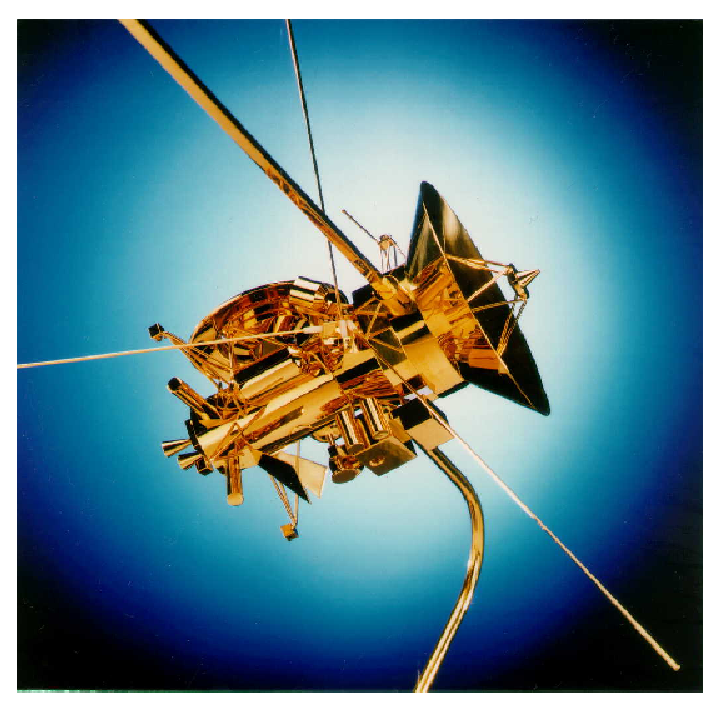
\includegraphics[width=0.8\linewidth]{paperpics2/fig1b.eps}
\caption{The 1:30 scale model of Cassini with the RPWS antenna system.\label{fig1b}}
\end{figure}

\begin{figure}
\centering
  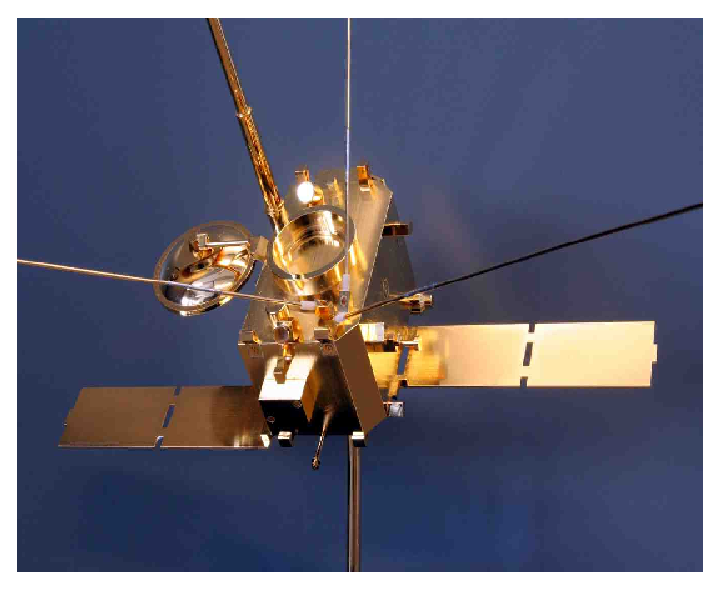
\includegraphics[width=0.8\linewidth]{paperpics2/fig1c.eps}
\caption{The STEREO antennas have already observed a Type III solar radio burst(oct. 30,2006).\label{fig1c}}
\end{figure}

\begin{figure}
\centering
  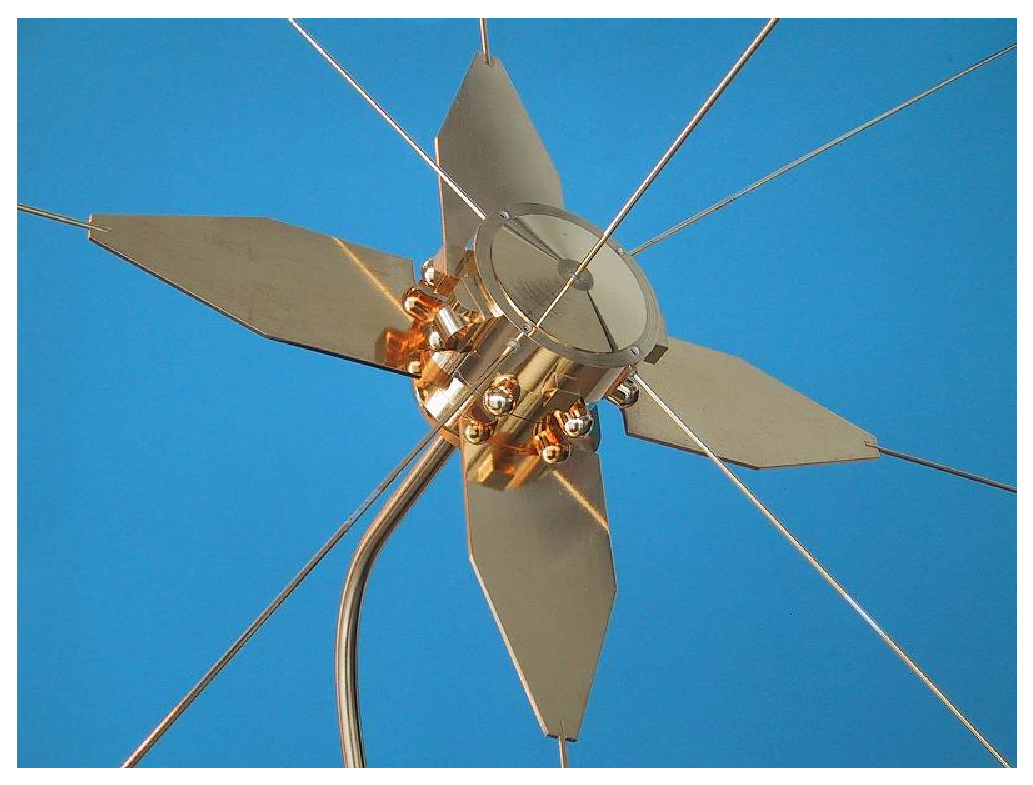
\includegraphics[width=0.8\linewidth]{paperpics2/fig1d.eps}
\caption{The INTERBALL antenna system (inbetween the solar panels) has observed terrestrial AKR.\label{fig1d}}
\end{figure}

As indicated below a series of spacecraft antenna systems have already been calibrated using scale models for rheometry measurements. In Figures \ref{fig1b}, \ref{fig1c}, \ref{fig1d} models of the Cassini spacecraft, STEREO, and INTERBALL are displayed.

\section{The numerical method}
\subsection{Technical aspects}
The numerical method for determining the relevant antenna properties is based on electromagnetic codes. At first, a wire-grid model of the spacecraft is constructed (see Figure \ref{fig2}). Then, numerical codes are used to get the current distribution on the surface of the antenna-spacecraft system.

\begin{figure}
\centering
  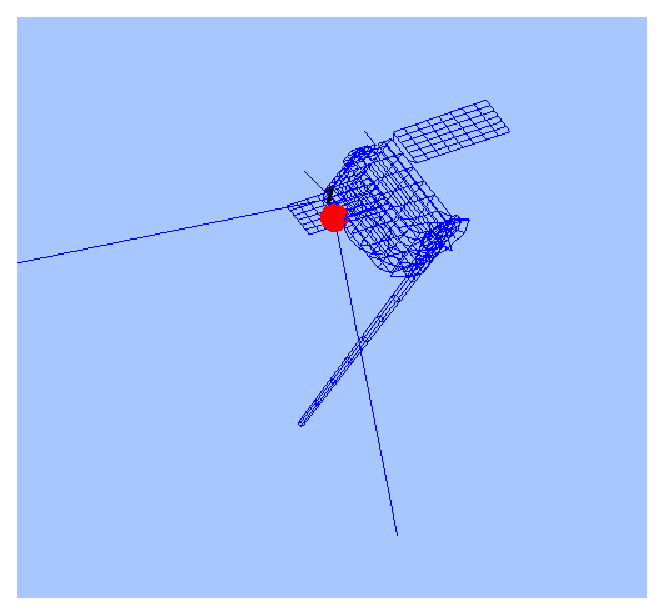
\includegraphics[width=1.0\linewidth]{paperpics2/fig2.eps}
\caption{The wiregrid model of STEREO.\label{fig2}}
\end{figure}

Calculation of the current distribution on the surface of the spacecraft is done by application of two programs:

\begin{itemize}
    \item The Antenna Scatterers Analysis Program (ASAP) is an open source program, using the method of moments (MOM) to solve the reaction integral equation. As representation of the currents, a piecewise sinusoidal expansion is used.
\item CONCEPT II is a proprietary software written at the University of Hamburg-Harburg. It uses the MOM to solve the electric field integral equation (EFIE) and uses triangular base functions to represent the currents.\end{itemize}


In the regime of the spacecraft antennas both programs are equally valid, so the consistency of the two results is a good indication for the validity of the method and the modeling process. In both cases  the antennas are excited by an electromotive force of 1V at the feed points. One of the feeds is marked by the red dot in Figure \ref{fig2}. Only currents along the wires are considered, all transverse currents are ignored. Another simplification made is that the currents are infinity thin and flowing along the center of each wire.

The integral equations have to be solved in conjunction with the boundary conditions. Both programs use the MOM which was developed in this form by Roger Harrington \cite{harrington}. The integral equation is transformed into a matrix equation which can be solved by means of linear algebra.
Based on the currents along the wires, the effective length vectors, the fields, the radiation pattern and the impedances can be computed. This is done by using Matlab functions. The main advantage of this method is flexibility with regard to the representation of spacecraft parts, which can easily be altered to test their influence on antenna properties.

\subsection{Constraints}
The application of wire-grid modeling for the calibration of an antenna system is naturally constraint by some facts given in the following:

\begin{itemize}
    \item The numerical method is suitable for a frequency from approximately 300kHz up to a frequency where one of the following conditions are no longer fulfilled:
\begin{itemize}
    \item The wavelength must be considerably longer than the longest wire-segment.
\item The mesh size must be considerably smaller than the wavelength.\end{itemize}
\item Below this frequency range numerical instabilities may occur due to the ill conditioning of the resulting matrix. Above this range the wire-grid model is not suitable to model the spacecraft accurately enough.
\item Another limitation regards the relation of the segment length to the segment diameter. This relation has to be large enough in a way that it represents a wire rather than a cylinder.
\item The limitation on the number of segments is given in form of the computation time. At the moment we work with a number of segments of 1000-1500, which can easily be handled by common PCs.
\end{itemize}



\section{The experimental method}
\subsection{Technical aspects}
Rheometry is an experimental technique to determine the effective length vectors of antennas in the quasi-static frequency range, where the wavelength is much greater than the dimension of the antenna system. Its advantages are that the antenna system (antennas as well as spacecraft) can be modeled in great detail and that the used measurement set-up is pretty much disturbance-free, contrary to the standard high-frequency measurements.

\begin{figure}[b]
\centering
  \includegraphics[width=1.0\linewidth]{paperpics2/fig3.eps}
\caption{The rheometry setup (adapted from \cite{rheometry}).\label{fig3}}
\end{figure}

A gold plated model of the antennas-spacecraft system has to be built. This model is immersed in an electrolytic tank (see Figure \ref{fig3}). Metal plates are attached to two opposite sides of the tank to form a large capacitor. A signal generator is connected to the plates to sustain a homogeneous electric field in the tank. The voltages at the model antennas are measured as a function of the model orientation. For that purpose the model can be rotated around a vertical axis, and different suspensions of the model at this axis are used. So the induced voltages for a variety of orientations of the model with regard to the electric field direction are recorded, from which the effective length vectors can be inferred.

\subsection{Constraints and pros}
Rheometry is suitable for consideration from the quasi-static limit up to a frequency where the effective length vectors are still constant and real. This limit is approximately 1.5MHz in case of the STEREO spacecraft. At these low frequencies there may be problems with the numerical method due to the ill conditioning of the resulting matrices. An advantage of the rheometry is that very fine details of the spacecraft body can be modeled, whereas numerical methods soon reach their limit when small parts near the antenna feed zone have to be modeled.

\section{Conclusion}
Either method has its own advantages. Rheometry can be far more detailed compared with wire-grid simulations, so the influence of the fine structure of the spacecraft can be estimated by comparison of the two methods. Rheometry is therefore a good basis to decide about improvements of wire-grids, it further yields a purely quasi-static result, which must agree with the asymptotic limit of the numerical calculations as the frequency converges to zero. The advantage of the computer simulation is the flexibility regarding the model structure, so it can be used to study the perturbation of antenna properties provoked by single spacecraft parts. Of course, the decisive advantage is that electromagnetic codes are devised for high-frequency analysis up to frequencies far above the resonance, thereby enabling the estimation of the validity range of the quasi-static results.





\section*{Acknowledgments}
These studies were supported by the Austrian Space Applications Programme (ASAP).



   \bibliographystyle{aa}
   \bibliography{../../Bibliography/MyBib}

\end{document}
%%
%% <<<<< End of generated file <<<<<<
%%
%% End of file `esapub.tex'.
